\newpage
\section{Algoritmo Propuesto}\label{sec:algoritmo}
\subsection{Explicaci\'on}

\subsubsection{Colonia de hormigas}

El algoritmo implementado esta basado en la metaheur\'istica de \textbf{colonia de hormigas}.

La idea general es tener una matriz que representa a la \textbf{feromona}, esta matriz reprensenta la region de entrada, en otras palabras el valor en la posicion (x,y) de la matriz de feromona representa el valor de la feromona en dicha posicion del suelo. En un principio se inicaliza con todos los valores en 0, como se ve a continuacion:


\begin{center}
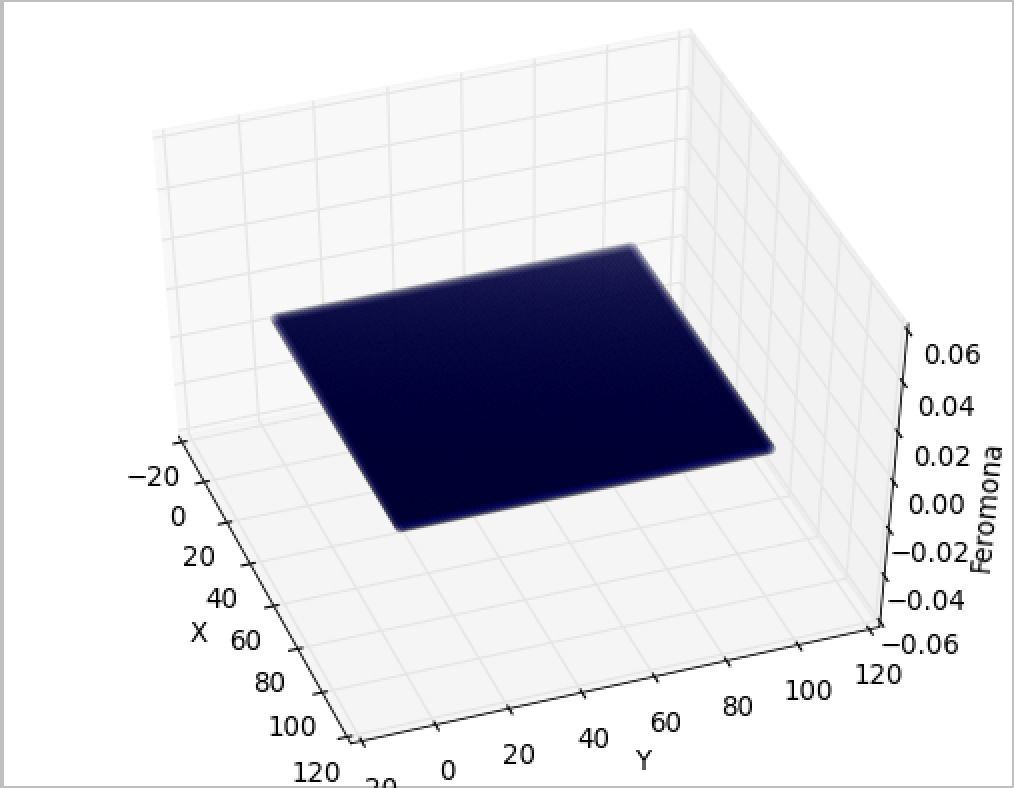
\includegraphics[width=7cm]{imagenes/feromona0}
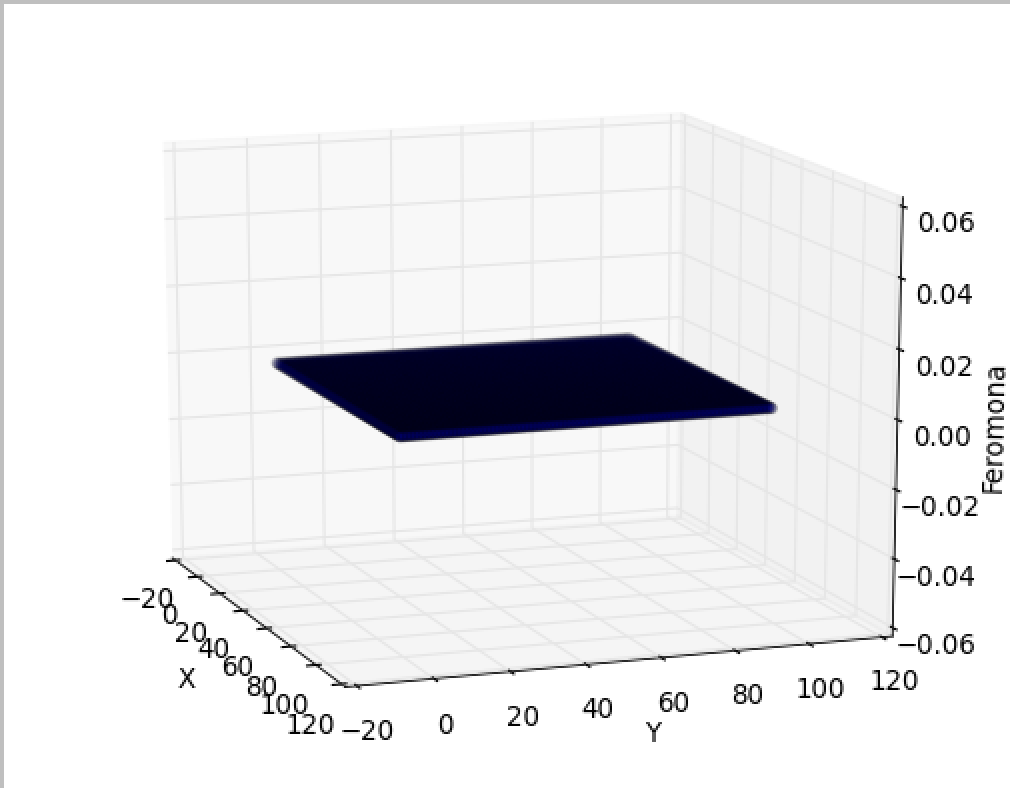
\includegraphics[width=7cm]{imagenes/feromona01}
\end{center}

La matriz de fermona esta \textbf{discretizada} con un valor \textbf{configurable por par\'ametro}. Por ejemplo, si la regi\'on es de 100x100 metros, pero la discretizacion de la feromona la seteamos en 10 metros, vamos a tener una matriz de feromona de 10x10. Es clave notar en este punto que cuanto menor es el valor de la discretizaci\'on de la feromona mayor cantidad de puntos en la matriz y por lo tanto vamos a lograr mejores resultados pero a su vez resultados con tiempo computacional m\'as alto (ver secci\'on de experiemntaci\'on).

Por otro lado, contamos con una estructura auxiliar, una matriz de tamaños iguales que la matriz de feromona, esta estructura contiene 0 y 1 dependiendo de la \textbf{disponibilidad} del punto de la feromona. Esto es utilizado para saber cuando una feromona esta disponible, dado que los vamos a ir tapando con el correr de las iteraciones y por otro lado, en casos de que la regi\'on original no sea rectangular o este rotada, la matriz de feromona se arma de forma tal que la regi\'on quede incluida y los espacios fuera de la regi\'on se setean como \textbf{no disponibles} en esta nueva estructura. 

En la siguiente figura vemos un ejemplo donde la seccion amarrilla seria la regi\'on, y la azul seria la matriz de feromona, por lo tanto en la matriz de disponibilidad en los casilleros correspondientes a partes azules tendriamos un 1 indicando que no esta disponible esa feromona, ya que no esta dentro de la regi\'on.

\begin{center}
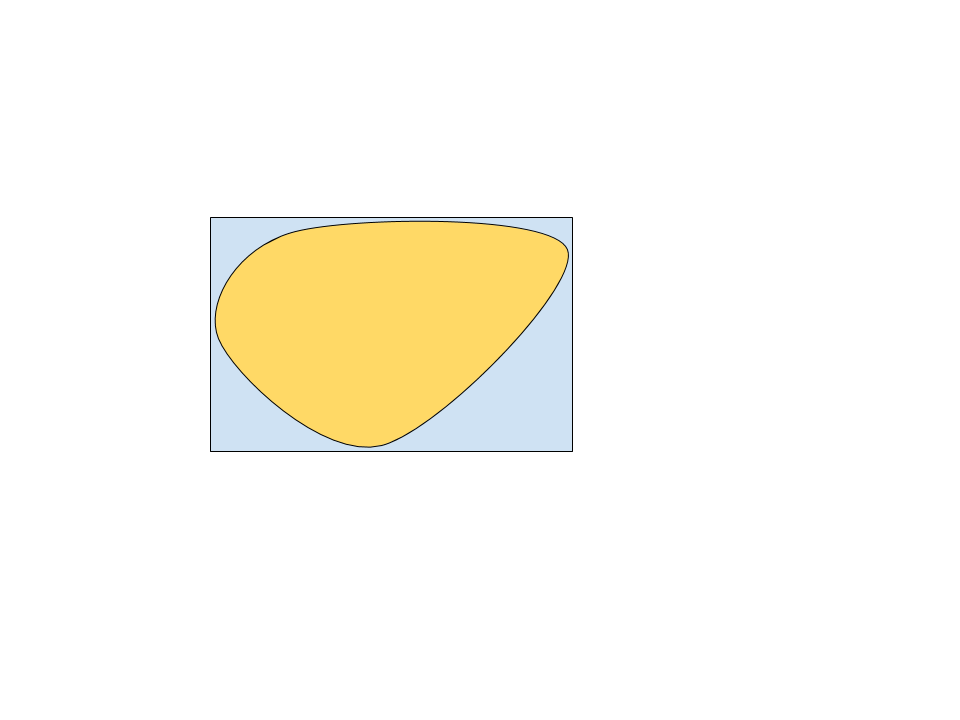
\includegraphics[width=6cm]{imagenes/ejemplo1}
\end{center}


Lo siguiente es, ejecutar una cantidad configurable de iteraciones el algoritmo obteniendo en cada soluci\'on, un conjunto de soluciones que van \textbf{actualizando} la matriz de feromona y en cada paso del algortimo vamos \textbf{chequeando y guardandonos la mejor soluci\'on}, siendo la mejor soluci\'on la que tenga el valor m\'as alto del ogip tapado. 

\newpage

En las siguientes imagenes podemos ver algunos ejemplos de feromonas luego de varias iteraciones.

\begin{center}

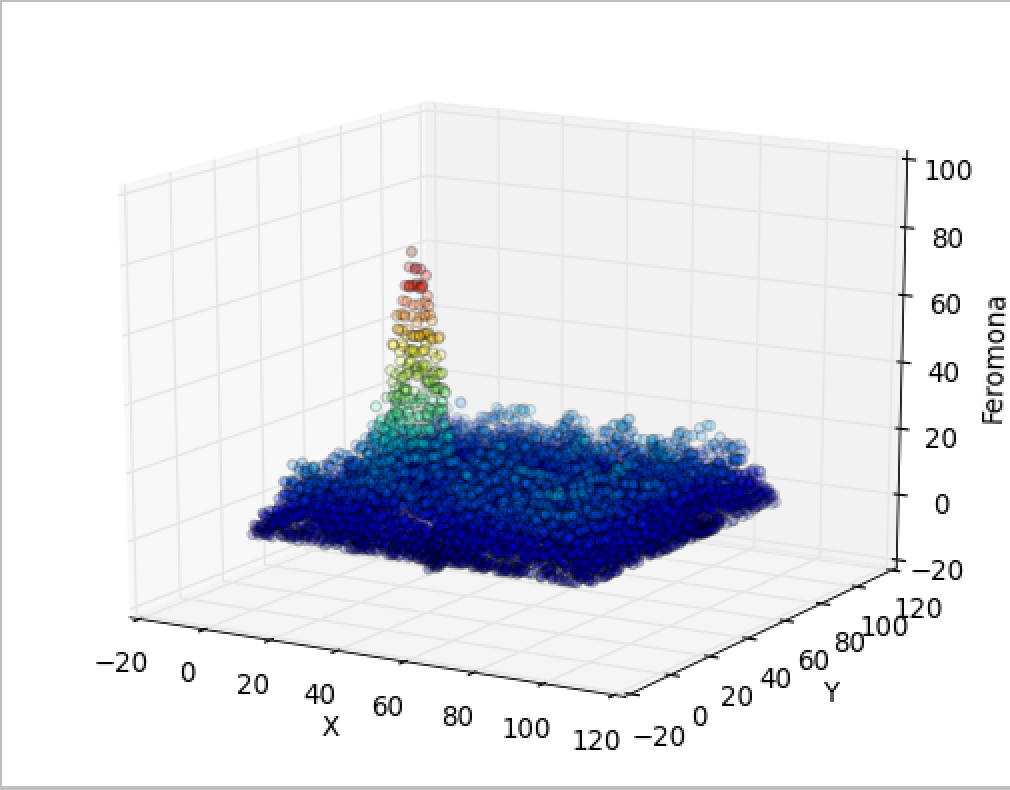
\includegraphics[width=7cm]{imagenes/fero0}
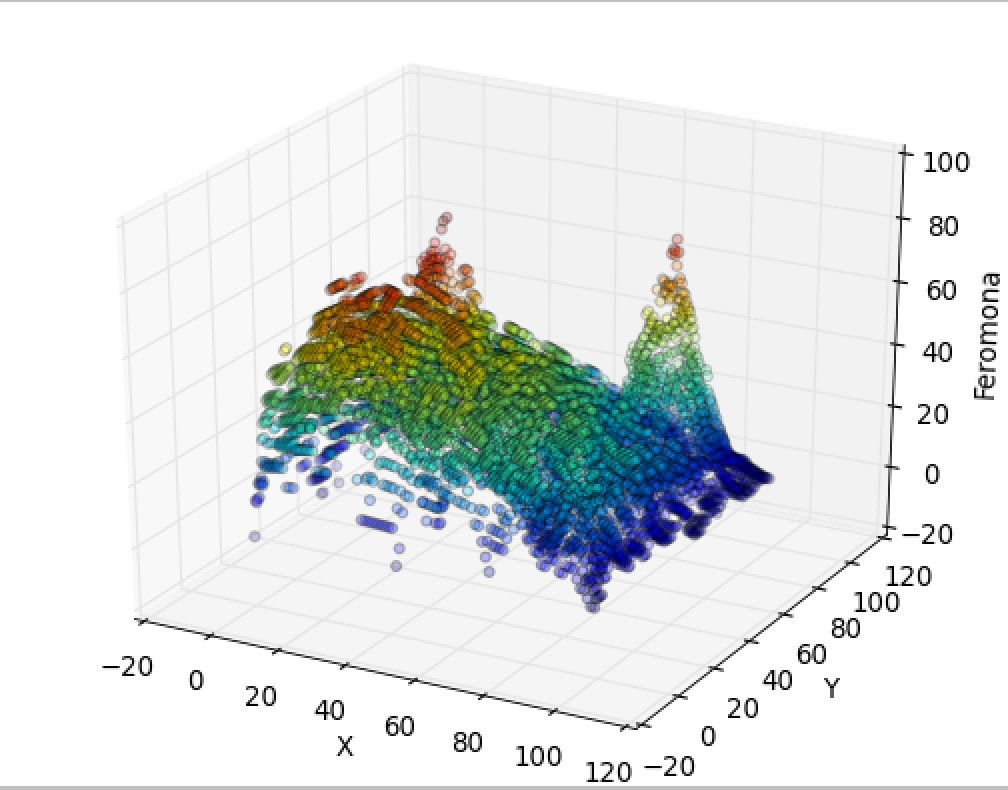
\includegraphics[width=7cm]{imagenes/fero1}
\end{center}


El algoritmo esta dividido en dos partes, la \textbf{iteraci\'on inicial} y el \textbf{resto de las iteraciones} (decisi\'on tomado para facilitar la implementaci\'on). 

A continuaci\'on se explica el trabajo de cada hormiga, es decir la forma de conseguir cada soluci\'on dependiendo si es la iteraci\'on inicial o el resto de las iteraciones.

\textbf{Iteraci\'on Inicial:} En esta iteraci\'on se crean una \textbf{cantidad configurable} de soluciones random, y para cada una de estas se actualiza la matriz de feromonas de la forma que corresponda. 

Para crear una soluci\'on random, la idea principal es meter pads centrados en puntos random de la regi\'on, teniendo en cuenta que sean v\'alidos (que esten dentro de la regi\'on, sin pisarse y sin interceptarce con una restrinci\'on) hasta no poder meter mas pads. Notar que tambien se elije la semilla de forma random. El problema en este caso es decidir cuando ya no se pueder meter pads (dado que estamos trabajando en un plano \textbf{continuo}), por lo tanto se considero tener un \textbf{valor configurable} de intentos de meter pad fallidos. En caso de fallar en insertar el pad random esa cantidad de veces entonces se considera que no entra ning\'un pad mas y se retorna la soluci\'on. 

A continuaci\'on podemos ver un ejemplo de una soluci\'on random, donde termino de poner pads porque se \textbf{creyo} que no entraban mas, pero podemos ver en la otra figura, marcado con amarrillo 3 posibles pads que se nota que no se encontraron.

\begin{center}
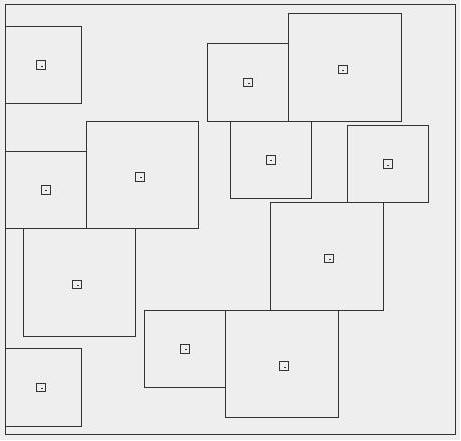
\includegraphics[width=7cm]{imagenes/ejemplo2}
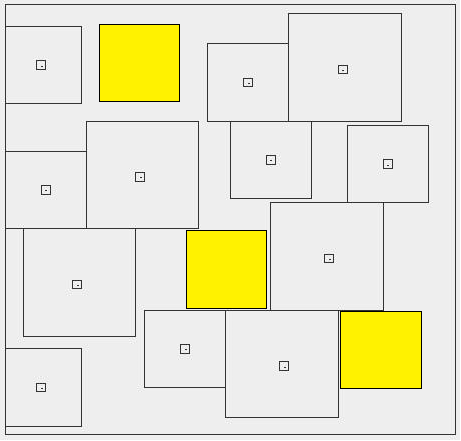
\includegraphics[width=7cm]{imagenes/ejemplo3}
\end{center}




\textbf{Resto de las iteraciones:} En esta iteracio\'n se crean una \textbf{cantidad configurable} de soluciones no random, y para cada una de estas se actualiza la matriz de feromonas de la forma que corresponda.

Para crear una \textbf{soluci\'on no random}, la idea principal es agarrar el punto de la feromona m\'as \textbf{caliente} y generar una \textbf{cantidad configurable} de pads random que puedan tapar esa feromona. 

Nota: si no consigo ningun pad random que tape dicho punto de la feromona (dado que los pads pueden ser invalidos, por ejemplo tocando una restriccion) , descarto ese punto de la feromona. 


La manera de conseguir un pad random que tape un punto c, es tan simple como un pad posicionado en cualquier lugar de la regi\'on que tape a c. \textbf{Esto esta hecho de esta forma para que cada soluci\'on sea distinta de las otras.}

Una vez tapado el punto de la feromona, se acomoda el pad, se tapan el resto de los puntos de la feromona que este pad tapo (tambi\'en actualizamos la matriz de disponibilidad) y se itera hasta no tener m\'as puntos feromona para tapar. 

\textbf{Actualizaci\'on de la feromona:} Para actualizar la feromona utilizamos una funci\'on llamada \textbf{esBuenasoluci\'on} que determina si una soluci\'on es buena o mala. Contamos con un \textbf{par\'ametro configurable} dado que se tiene 3 formas distintas de ver si una soluci\'on es buena o mala

\begin{enumerate}
\item Opci\'on 0: Una soluci\'on es buena si el ogip cubierto por esta soluci\'on es mas que el 75\% del total del ogip, en otro caso es una mala soluci\'on.
\item Opci\'on 1: Una soluci\'on es buena si el ogip cubierto por esta soluci\'on es mas que la mitad de la suma del maximo y minimo ogip hasta el momento, en otro caso es mala soluci\'on.
\item Opci\'on 2: Una soluci\'on es buena si el ogip cubierto por esta soluci\'on es mas que el promedio de los ogip de las soluciones calculadas hasta el momento, en otro caso es mala soluci\'on. 
\end{enumerate}

En caso de que la soluci\'on sea buena se recorre la matriz de feromonas, aumentanto (calentando) en cada casillero (punto de la feromona) tapado por un pad en dicha soluci\'on un valor igual al ogip en ese punto (normalizado) por una constante configurada por parametro. Es analogo para el caso de una soluci\'on mala, solamente que disminuyendo (enfriando).


\textbf{Importante:} Tener en cuenta que para todos los casos, una vez elegido el pad que voy a agregar a mi soluci\'on, a este pad lo \textbf{acomodo} haciendo que se mueva para la direccion mas cercana a otro pad o borde, hasta chocarce con el. De esta forma obtengo soluciones con pad pegados entre si y no aparecen huecos.

Una vez terminadas todas las iteraciones vamos a tener guardado la mejor soluci\'on, el n\'umero de iteracion de donde sali\'o dicha soluci\'on y el tiempo en conseguirla.

Notar que la mejor soluci\'on no necesariamente es de la \'ultima iteraci\'on, es por eso que la vamos guardando en cada iteraci\'on y tambi\'en vamos guardando el n\'umero y tiempo de la iteraci\'on de donde se origin\'o la mejor soluci\'on.

\subsubsection{Colonia de hormigas Versi\'on Alternativa}

Tambi\'en se desarrollo un algoritmo extra, tambi\'en basado en \textbf{colonias de hormigas}, implementado de forma casi identica al anterior, salvo que en lugar de tener una \'unica matriz de feromonas, tenemos una matriz de feromonas por cada semilla, es decir si tengo 5 semillas (tipo de pad) tengo 5 matrices de fermona y una \'unica matriz de disponibilidad. 

Entonces a la hora de actualizar la matriz de feromona, actualizamos para cada matriz los puntos tapados por los pads que tienen esa semilla. Por ejemplo, si tenemos 2 semillas, una grande y una chica, en una matriz de feromona vamos a actualizar los puntos tapados por los pads chicos y en la otra matriz de feromona actualizamos los puntos tapados por pads grandes. 

A la hora de buscar la feromona m\'as caliente, se busca entre todas las matrices de feromona.

El objetivo de esto es notar la variaci\'on de la feromona, y tratar de ver que en algunos casos es conveniente poner los pads mas grandes en los puntos mas calientes mientras que los lugares restantes, por ejemplo a los costados de los lugares de alto valor, se agregan pads mas chicos. 

\newpage

A continuaci\'on se muestran ejemplos de feromonas para esta versi\'on alternativa. Podemos ver en la figura de la izquierda como se modific\'o la feromona en los lugares donde tiene los pads mas grandes. Por otro lado, la feromona de la derecha se nota como esta modificada en los lugares que rodean a los pads mas grandes, concluyendo que se pusieron pads mas chicos en los alrededores de los mas grandes (ver secci\'on experiementaci\'on)

\begin{center}

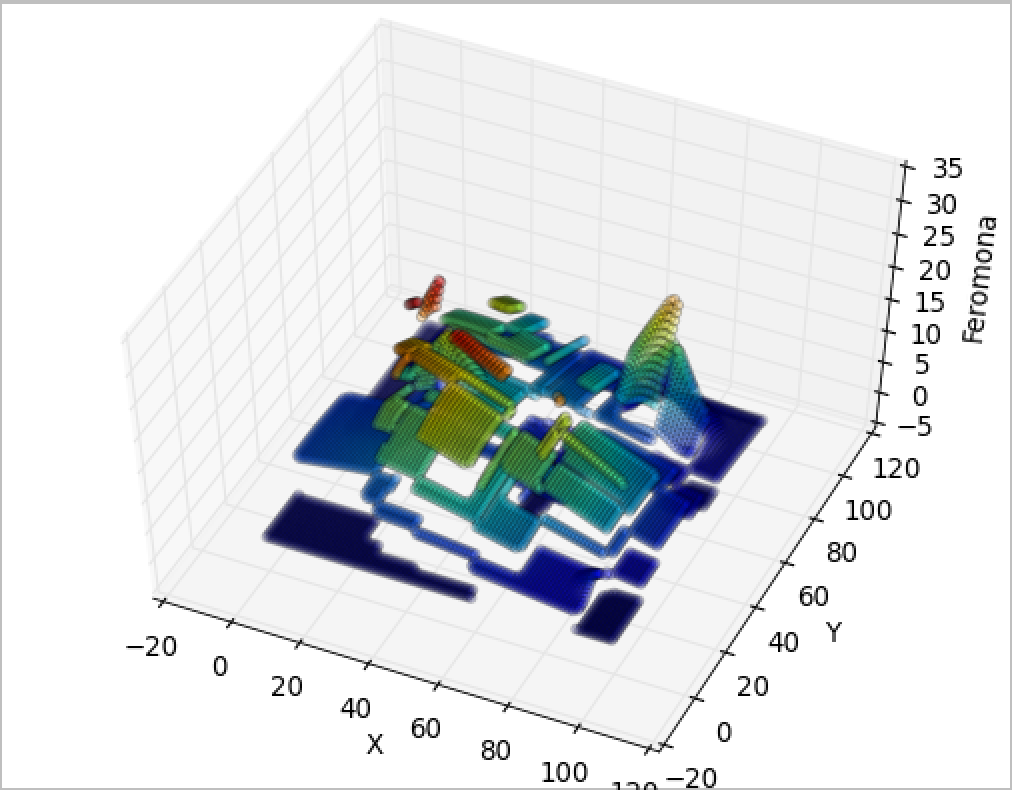
\includegraphics[width=7cm]{imagenes/ferov20}
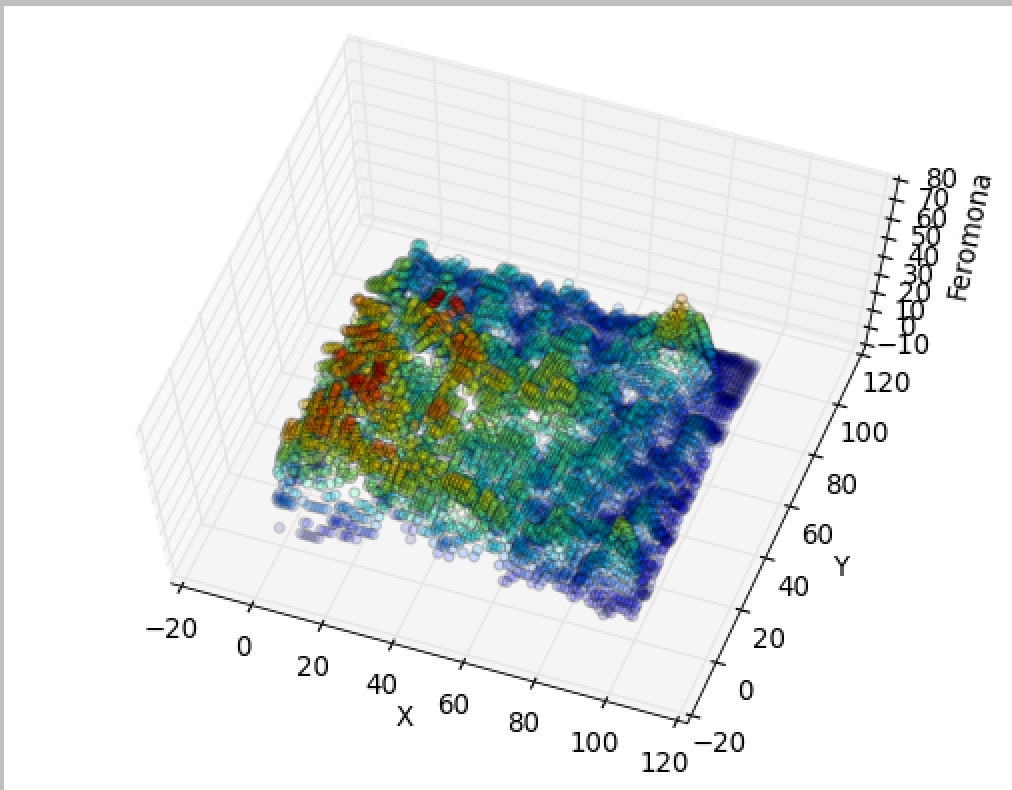
\includegraphics[width=7cm]{imagenes/ferov21}
\end{center}

A continuaci\'on podemos ver algunos ejemplos de soluciones obtenidas sobre una misma instancia cambiando los par\'ametros (ver m\'as en secci\'on experimentaci\'on).

\begin{center}

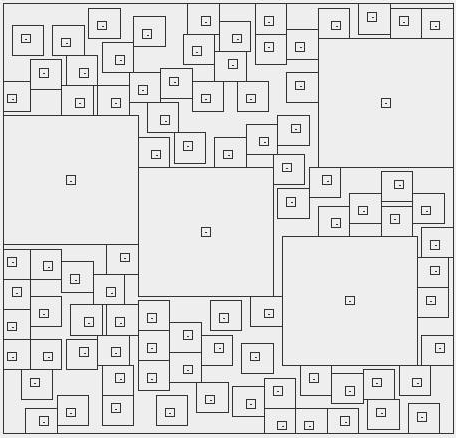
\includegraphics[width=7cm]{imagenes/ejemplo7}
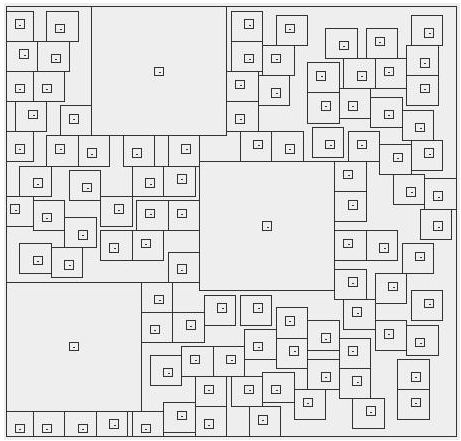
\includegraphics[width=7cm]{imagenes/ejemplo5}
\end{center}


\begin{center}
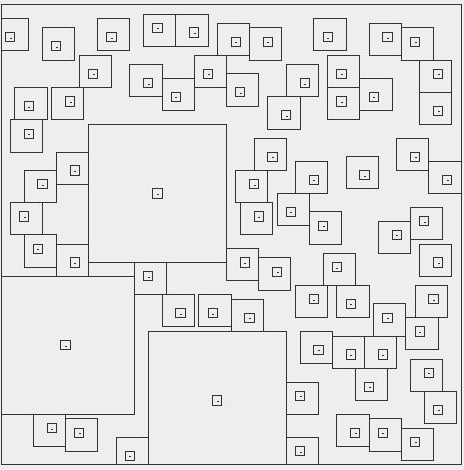
\includegraphics[width=7cm]{imagenes/ejemplo6}
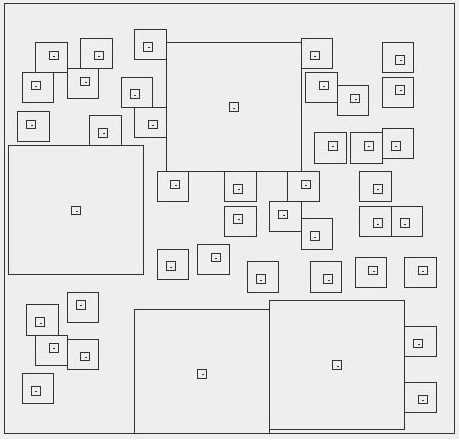
\includegraphics[width=7cm]{imagenes/ejemplo4}

\end{center}

Notar que en los dos primeros casos no quedaron huecos mientras que en los \'ultimos dos si, esto se debe a la discretizaci\'on de la feromona (en los \'ultimos dos casos la discretizacion es un n\'umero m\'as alto, por lo tanto tenemos menos lugares que tapar, provocando huecos).

\newpage


\subsection{Pseudocodigo}
\subsubsection{Algoritmo principal}

\begin{verbatim}
    resolver() {
        inicializarFeromonas();
        ejecutarIteracionInicial();
        return ejecutarProximassoluciones();
    }
\end{verbatim}

\textbf{InicializarFeromonas()} es una funci\'on que inicializa la feromona como una matriz del tamaño de la regi\'on, en caso que la regi\'on no se rectangular la inicializa con el rect\'angulo mas chico que contenga a la regi\'on. 

Tambi\'en inicializa una matriz disponibilidad del mismo tamaño que la feromona pero esta contiene 1 o 0 dici\'endonos si una feromona es validad o no, sea porque ya esta usada o porque la regi\'on es m\'as chica que la matriz de feromonas y en esa feromona no tenemos regi\'on.


\begin{verbatim}
    ejecutarIteracionInicial() {
        soluciones = crearsolucionesRandom();
        for (soluci\'on soluci\'on : soluciones) {
            if(esBuenasoluci\'on()){
                actualizarFeromona(soluci\'on, OperacionFeromona.Calentar);
            } else {
                actualizarFeromona(soluci\'on, OperacionFeromona.Enfriar);
            }
        }
    }
\end{verbatim}		

\textbf{ejecutarIteracionInicial()} crea una cantidad seteada por par\'ametro de soluciones randoms y para soluci\'on chequea si es una buena o mala soluci\'on, la funcion \textbf{esBuenasoluci\'on()} cambia seg\'un un valor pasado por parametro, pero en definitiva, devuelve \textbf{true} si es una soluci\'on considerada buena o \textbf{false} si es considerada mala. 

En caso de que la soluci\'on sea buena, \textbf{calentamos} la matriz de feromonas y \textbf{enfriamos} en caso contrario.

La funci\'on \textbf{actualizarFeromona()} simplemente recorre la matriz \textbf{calentando} o \textbf{enfriendo} cada valor respectivamente. Pero notar que la calienta \textbf{teniendo en cuenta el valor del ogip en ese punto}, es decir, se normaliza el ogip y en cada punto de feromona se calienta o enfr\'ia un valor igual a $escalar * feromonaNormalizadaEnElPunto$. Esto es para que el algoritmo de colonias de hormigas tenga en cuenta los valores originales del problema para generar sus soluciones.


La funci\'on \textbf{esBuenasoluci\'on()}, tiene 3 opciones que se cambian dependiendo de un valor pasado por par\'ametro

\begin{enumerate}
\item Opci\'on 0: Una soluci\'on es buena si el ogip cubierto por esta soluci\'on es mas que el 75\% del total del ogip, en otro caso es una mala soluci\'on.
\item Opci\'on 1: Una soluci\'on es buena si el ogip cubierto por esta soluci\'on es mas que la mitad de la suma del m\'aximo y m\'inimo ogip hasta el momento, en otro caso es mala soluci\'on.
\item Opci\'on 2: Una soluci\'on es buena si el ogip cubierto por esta soluci\'on es m\'as que el promedio de los ogip de las soluciones calculadas hasta el momento, en otro caso es mala soluci\'on. 
\end{enumerate}

\newpage

\begin{verbatim}	
crearsolucionesRandom() {
    ret = new soluci\'on()
    while (hasta que el area deje de cambiar) {
        Coordenada c = generarCoordenadaRandom()
        Pad pad = crearPadConSemillaRandamCentradaEnCoordenada(c)
        if (padValido(pad)){
            Pad padAcomodado = acomodarPad(pad);
            agregarPadAsoluci\'on(ret,padAcomodado);
        }
    }
    return ret;
}
\end{verbatim}	

La condici\'on del while corta cuando ya no se pueden meter mas pads en mi soluci\'on random, esto se hace teniendo en cuenta una cantidad fijada por parametro de intentos de meter un pad, es decir, intento meter pads en la soluci\'on y si la cantidad de veces que no pude meter es mayor al par\'ametro seteado, se asume que no entran m\'as pads y sale del while. 

Esto se hace para tratar de manejar la regi\'on en un plano \textbf{continuo} y para tratar de solucionar el problema de saber cuando ya no entran mas pads.

\textbf{GenerarCoordenadaRandom()} generada un x,y random dentro de la region. 

\textbf{crearPadConSemillaRandamCentradaEnCoordenada(c)()} elije una semilla random y crea un pad centrado en c

\textbf{padValido(pad)} chequea si el pad no se pisa con ninguna restricci\'on, ni se va fuera de la regi\'on, ni se pisa con otro pad ya agregado a la soluci\'on.

\textbf{acomodarPad(pad)} mueve el pad para una direcci\'on random hasta chocarse son un borde u otro pad sin destapar el centro. Eso se hace para tratar de pegar todos los pads en la soluci\'on.

\textbf{agregarPadAsoluci\'on()} agrega el pad a la soluci\'on.

\textbf{ejecutarProximassoluciones()} ejecuta una cantidad de veces igual a \textbf{cantIteraciones}, un algoritmo similar a \textbf{crearsolucionesRandom()}, llamado \textbf{generarsolucionesMaximaTemperatura()}. De esta forma se crean soluciones durante muchas iteraciones.

\textbf{generarsolucionesMaximaTemperatura()} es exactamente igual a \textbf{crearsolucionesRandom()} nada mas que cambiando el m\'etodo \textbf{crearsolucionesRandom()} por \textbf{generarsolucionesMaximaFeromona()}. Esto significa que crea una cantidad configurable de soluciones de m\'axima feromona. Y para cada soluci\'on chequea si es buena o mala actualizando la feromona como corresponda al igual que lo hac\'iamos en la iteraci\'on inicial.

Una soluci\'on de m\'axima feromona es una soluci\'on que tiene en cuenta el valor de la fermona para generarse y se genera con el siguiente algoritmo:


\begin{verbatim}
construirsoluci\'onMaximaTemperatura() {
    sol = new soluci\'on();
    while (mientra que tenga feromonas disponibles) {
        Feromona p = getMaximaFeromona()
        if (es una feromona que se puede tapar) {
            for (int j = 0; j < getCantIntentosTaparFeromona(); j++) {
                nuevoPad = generarNuevoPad(p);
                if (esPadValido(nuevoPad)) {
                    nuevoPad = acomodarPad(nuevoPad);
                    agregarPadAsoluci\'on(nuevoPad);
                    break;
                }
            }
        }
    }
    return sol;
}
\end{verbatim}

Mientras tenga feromonas disponible, es decir que todavia no las tapas (y est\'an dentro de la regi\'on) ejecuto todo el c\'odigo dentro del while. 

Obtengo la m\'axima feromona con \textbf{getMaximaFeromona()} y chequeo si es una posible feromona a tapar, dado que podr\'ia pasar que esa feromona este en una restricci\'on. 
Una vez que ya se que esa feromona la puedo tapar, trato de generar \textbf{getCantIntentosTaparFeromona()} pads (este valor es seteado por parametro). 

La idea general es que para cada iteracion genero un pad random que tape a la feromona, chequeo si es valido, y si es valido lo agrego a la soluci\'on y dejo de intentar tapar esta feromona.

Si no encontre ningun pad que sea valido y tape a la feromona en \textbf{getCantIntentosTaparFeromona()} intentos entonces ya esa feromona la descarto. 

\textbf{Notar que a los pads los acomodo (al igual que antes) para que queden pegados a otros pads o al borde.}

\textbf{Nota importante:} Tanto en la generaci\'on de soluciones random o las soluciones de m\'axima feromona, a la hora de fijarse si es una buena o mala soluci\'on para actualizar la feromona, se chequea si es la \textbf{mejor soluci\'on}, en caso de ser la mejor se \textbf{guarda}. Esto es para guardar la mejor soluci\'on en el camino, podr\'ia llegar a pasar que la mejor soluci\'on la encuentre en iteraciones iniciales y las siguientes sean peores.


\subsubsection{Alternativa: Muchas Feromonas}
A parte de tener un algoritmo de colonias de hormigas que ejecuta con una \'unica feromona, se program\'o una versi\'on alternativa donde contamos con mas de una feromona. Es decir para cada soluci\'on, en lugar de tener una unica feromona, \textbf{tenemos una matriz de feromona para cada semilla}.
 
Para esto se modific\'o leventente el c\'odigo teniendo en cuenta que ahora manejamos arrays de feromonas, y cambian levemente los algoritmos de actualizar la feromona. En particular, el algoritmo para obtener c\'ual es la m\'axima feromona es el siguiente:


\begin{verbatim}
getMaximaFeromona() {
    result = null;
    for (f in todas las feromonas) {
        if(si la feromona f tiene valores dissponibles)
            if(maximo de f > result)
                result = f1;
    }
    return result;
}
\end{verbatim}

El algoritmo es bastante sencillo, la idea es recorrer todas las feromonas buscando el m\'aximo valor. 

Tener en cuenta que a la hora de actualizar la feromona, cada feromona solo se actualiza donde corresponde. Por ejemplo,  la feromona correspondiente a la semilla 0 se calienta o enfr\'ia solo en los puntos donde la soluci\'on puso semillas 0. 